\subsection{Star}%
\label{sub:star}
Ziel von Star ist die Berechnung von gecleanten Kamerabildern und die Berechnung
der Hillasparameter auf den Daten. 

\subsubsection*{Theorie}
image cleanining ist noetig weil, Bilder von falsch getriggerten PMTs
verrrauscht sind, diffuses Licht. Zur berechnung der Hauptachse werden dazu die
Bilder vom diffusen Untergrund befreit.
% Die Daten in einem getriggerten Event gehören nicht alle zu einem
% Tscherenkvoschauer.
% Um die folgenden Algorithmen zu verbessern,
% müssen Pixel, die nicht zum Schauer gehören, entfernt werden.

Dazu werden zur jeder anvisierten Quellposition (On-Position) ebensolange Daten
wo kein Gammafluss (Off-Daten) erwatet wird genommen.
Der Untergrund ist abhaengig von der Temperatur der PMTs welches mit
elektronischem Rauschen korreliert ist, der Wolkendecke, der observierten
Quellposition, ...
Mittels eines (likelihood test) wird der Untergrund verworfen.
Jeweils ein Beispiel für ein Kamerabild vor und nach dem Cleaning ist in
Abbildung~\ref{fig:cleaning} dargestellt.
\begin{figure}[htpb]
	\centering
	\begin{subfigure}[c]{0.35\linewidth}
		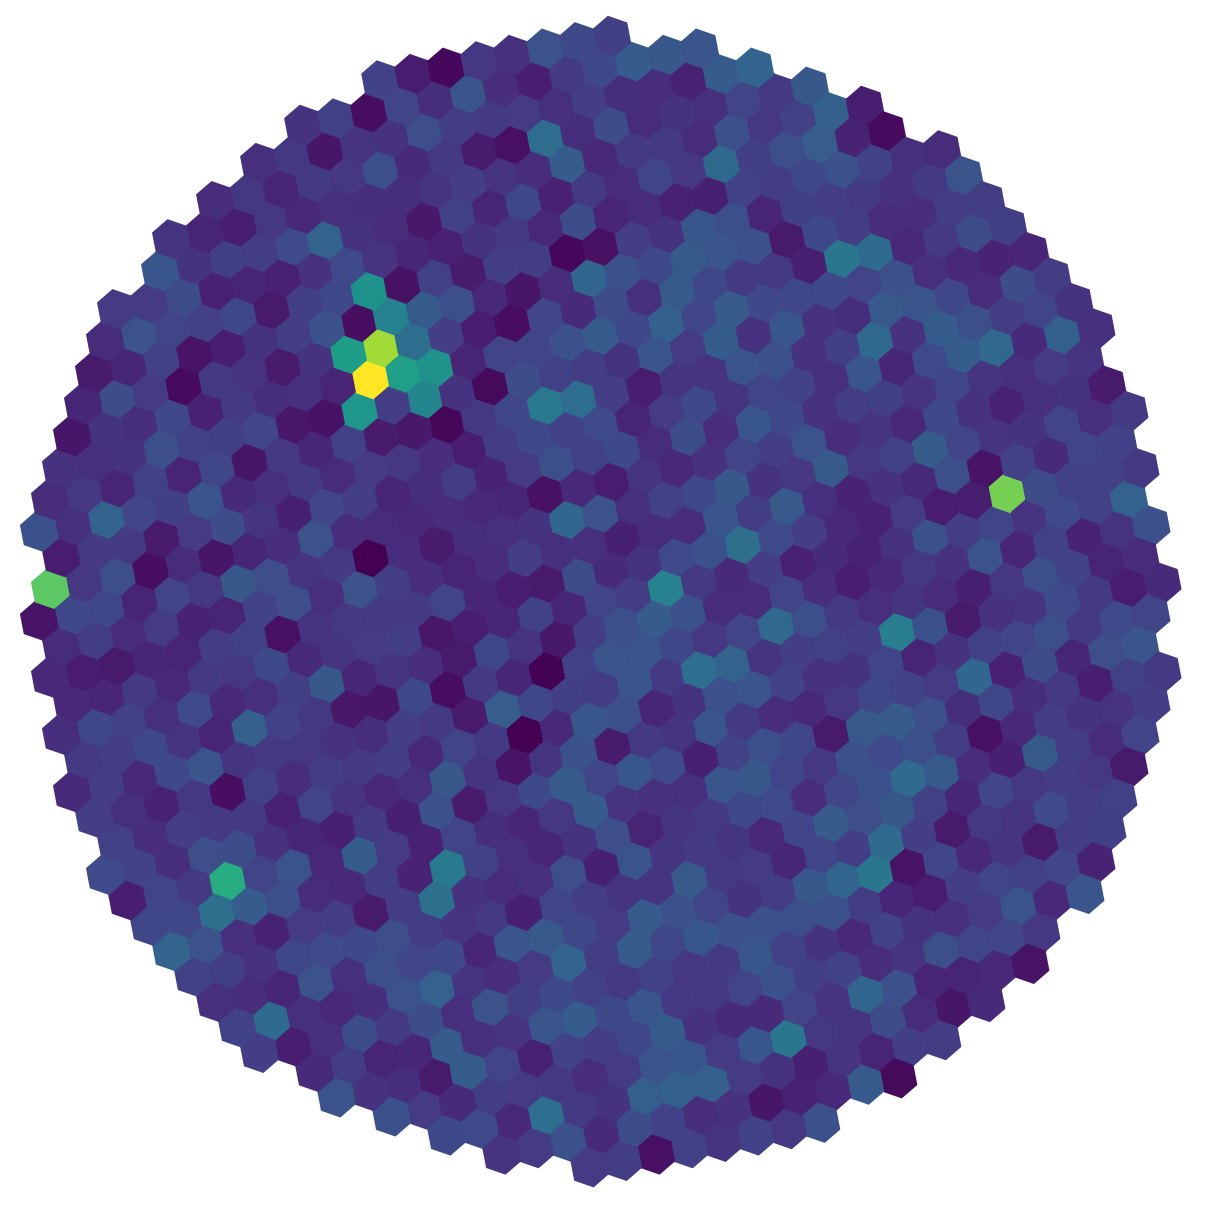
\includegraphics[width=\linewidth]{pictures/uncleaned.pdf}
		\caption{nicht bereinigte Daten}
		\label{fig:uncleaned}
	\end{subfigure}
	\begin{subfigure}[c]{0.35\linewidth}
		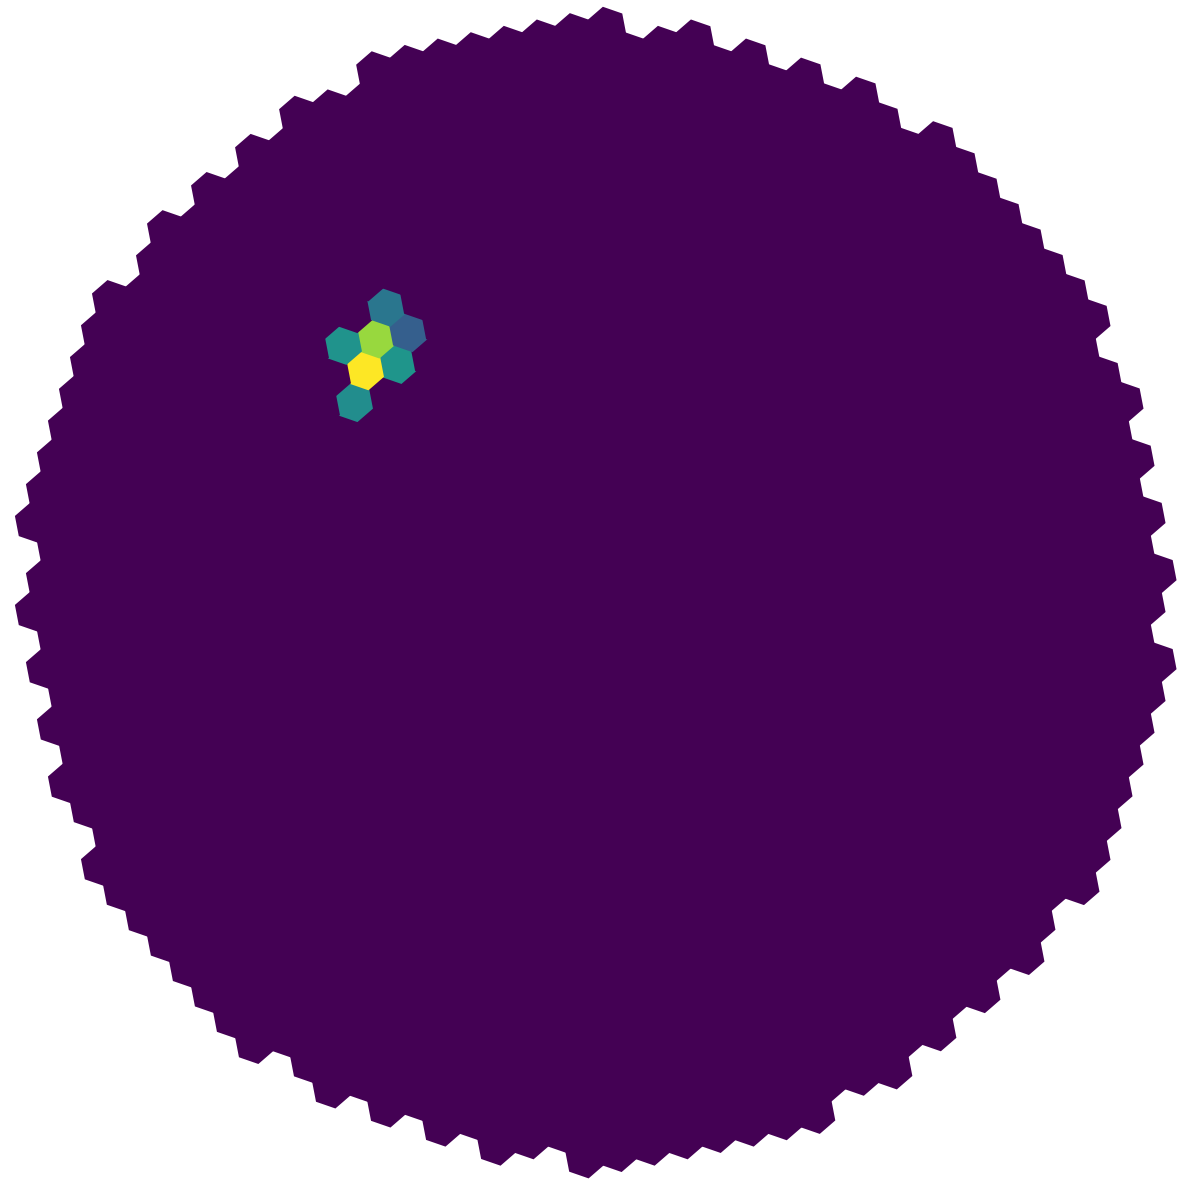
\includegraphics[width=\linewidth]{pictures/cleaned.pdf}
		\caption{bereinigte Daten}
		\label{fig:cleaned}
	\end{subfigure}
	\caption{Cleaning der Kamerabildern zur berrechnung der Hillas Parameter.}
	\label{fig:cleaning}
\end{figure}
Tscherenkvoschauer erzeugen in der Kamera Ellipsenförmige Events. 
Anhand der Größe der Ellipse und deren Richtung lässt sich die Energie des
Events bestimmen und die Richtung rekonstruieren.
Dazu wird auf den gecleanten Kamerabildern die Hillas Parameter bestimmt.

\begin{wrapfigure}[15]{o}{0.4\textwidth}
	\centering
	\includegraphics[width=0.8\linewidth]{tikz/build/hillas.pdf}
	\caption{Hillasparameter eines Schauers.}
	\label{fig:hillas}
\end{wrapfigure}
Die Hillas Parameter sind width, length, size, con core, disp und theta.
\textit{Width} ist die Nebenachse und \textit{length} die Hauptachse der Ellipse. 
\textit{Size} entspricht der Anzahl an Photonen die im Schauer detektiert wurden.
Da sich der Schwerpunk des Schauers in der Regel nicht mit dem Mittelpunkt der
Ellipse deckt ist dafür der Parameter \textit{Con Core} eingeführt.
Anhand der Parameter \textit{Size} lässt sich der Parameter \textit{dist}
schätzen der die Entferunung des Schauerschwerpunkt zur Rekonstruierten
Quellposition ist.
Die rekonstruierte Quellposition findet sich entsprechend der Orientierung der
Ellipse in einem Abstand von \textit{dist} von dem Schauerschwerpunkt entfernt.
Der Parameter \textit{theta} gibt an wie weit die rekonstruierte von der wahren
Quellposition entfernt ist.
123456789 Satz der noch ersetzt werden sollte damit man schauen kann ob die wrapfigure
richtig funktioniert und schoen aussieht.

\subsubsection*{Durchführung}
